\documentclass{article}
\usepackage{arxiv}

\usepackage[utf8]{inputenc}
\usepackage[english, russian]{babel}
\usepackage[T1]{fontenc}
\usepackage{url}
\usepackage{booktabs}
\usepackage{amsfonts}
\usepackage{nicefrac}
\usepackage{microtype}
\usepackage{lipsum}
\usepackage{graphicx}
\usepackage{natbib}
\usepackage{doi}
\usepackage{comment}
\usepackage{listings}
\usepackage{tabularx}




\title{Создание интеллектуальных систем}
\begin{comment}

\author{ David S.~Hippocampus\thanks{Use footnote for providing further
		information about author (webpage, alternative
		address)---\emph{not} for acknowledging funding agencies.} \\
	Department of Computer Science\\
	Cranberry-Lemon University\\
	Pittsburgh, PA 15213 \\
	\texttt{hippo@cs.cranberry-lemon.edu} \\
	%% examples of more authors
	\And
	Elias D.~Striatum \\
	Department of Electrical Engineering\\
	Mount-Sheikh University\\
	Santa Narimana, Levand \\
	\texttt{stariate@ee.mount-sheikh.edu} \\
	%% \AND
	%% Coauthor \\
	%% Affiliation \\
	%% Address \\
	%% \texttt{email} \\
	%% \And
	%% Coauthor \\
	%% Affiliation \\
	%% Address \\
	%% \texttt{email} \\
	%% \And
	%% Coauthor \\
	%% Affiliation \\
	%% Address \\
	%% \texttt{email} \\
}
\date{}

\renewcommand{\shorttitle}{\textit{arXiv} Template}

%%% Add PDF metadata to help others organize their library
%%% Once the PDF is generated, you can check the metadata with
%%% $ pdfinfo template.pdf
\hypersetup{
pdftitle={Создание интеллектуальных систем},
pdfsubject={q-bio.NC, q-bio.QM},
pdfauthor={David S.~Hippocampus, Elias D.~Striatum},
pdfkeywords={First keyword, Second keyword, More},
}

\end{comment}
\begin{document}
\maketitle

\begin{abstract}
	В данной работе решается задача предсказания FMRI по видео
\end{abstract}


\keywords{First keyword \and Second keyword \and More }

\section{Introduction}

В данной работе рассматривается задача прогнозирования следующего снимка FMRI (фМРТ, Функциональная магнитно-резонансная томография), по данным видео. FMRI – разновидность магнитно-резонансной томографии, которая проводится с целью измерения гемодинамических реакций (изменений в токе крови), вызванных нейронной активностью головного или спинного мозга. Этот метод основывается на том, что мозговой кровоток и активность нейронов связаны между собой. Когда область мозга активна, приток крови к этой области также увеличивается. FMRI позволяет определить активацию определенной области головного мозга во время нормального его функционирования под влиянием различных физических факторов (например, движение тела) и при различных патологических состояниях. Перечислим основные работы посвященные методам обработки FMRI.

В работе \cite{dataset} представлен один из самых обширных датасетов с данными (видео, FMRI).  Этот набор данных собран у большой группы испытуемых при просмотре одного и того же короткого аудиовизуального фильма. Датасет включает записи функциональной магнитно-резонансной томографии (фМРТ) (30 участников, возрастной диапазон 7-47 лет) во время выполнения одного и того же задания. Для аудиовизуального фильма представлены обширные аннотации (для звуковой и видеодорожки), такие как время появления / исчезоновения конкретных объектов, персонажей.

В работах \cite{fmri2} рассматриваются основные методы по работе с FMRI в задачах классификации. Одна из главных проблем и задач в обработке FMRI -- задача подавления шума, который возникает от движения головы, биения сердца, температурного шума и т.д. В работе предлагаются новые методы шумоподавления, выделения признаков с помощью топологического анализа данных, и показывается эффективность новых методов в задаче определения эпилепсии и депрессии.


Теперь мы рассмотрим методы обработки видео. В памяти компьютера видеосигнал хранится в виде последовательности кадров. Каждый кадр является цветной картинкой и представляется трёхмерной матрицей.

Естественным обобщенией сверточных сетей для работы с видео стало использование 3D свёрток. В отличие от 2D свёрток, которые успешно применяются для работы с отдельными изображениями, трёхмерные свёртки одновременно агрегируют информацию по времени и пространству. То есть свёртка применяется к перекрывающимся блокам, которые захватывают сразу несколько кадров. Недостаток 3D свёрток состоит в том, что они требуют больших вычислительных мощностей и сильно увеличивают количество параметров. Перечислим основные методы, позволяющие полностью или частично решить данную проблему. 

Первый подход предполагает использование двух отдельных моделей для обработки пространственной и временной информациии. Пространственная модель обрабатывает центральный кадр видеоряда, а временная получает на вход оптические потоки, причём ось времени переходит в ось каналов. Итоговое предсказание получают на основе эмбеддингов обеих моделей. Примеры  подхода можно найти в работах \cite{twostream}, \cite{inflated}. 

Второй подход основывается на факторизации 3D свёрток на 2D свёртки по пространству и 1D свёртки по времени. Чередовать свёртки малой размерности можно в разном порядке, а также применять параллельно, что отражено в \cite{fact3d}.

В статье \cite{inflated} был предложен другой способ ускорить сходимость модели, основанный на использовании предобученных 2D свёрток для хорошего начального приближения 3D свёрток.

Наконец, многие современные подходы полностью отказались от свёрток и учитывают пространственно-временные зависимости с помощью attention слоёв. Появились адаптации архитектуры Transformer для работы с видео (\cite{transformer}).

Так как наша цель состоит в предсказании fMRI по видео, то среди родственных задач следует выделить предсказание некоторого сигнала по исходному видеоряду. В частности, предлагается рассмотреть задачу video-to-video synthesis и предсказание аудио по видео.

Возможное решение первой задачи приведено в статье \cite{vidtovid}. Используется модель conditional GAN в предположениях Марковости: предсказания делаются только на основе предыдущих по времени значений исходного и сгенерированного сигнала. В функции потерь есть компонента, отвечающая за согласованность генерируемого сигнала.

В статье \cite{https://doi.org/10.48550/arxiv.2011.07340} решается задача озвучивания видео с помощью вариационного автоэнкодера. Во время обучения на вход подаётся последовательность кадров и звуковой сигнал. Сначала энкодер преобразует каждый кадр в вектор признаков, подающийся на вход реккурентной сети. Аналогичным образом обрабатывается звуковой сигнал. Реккурентные сети гененрируют среднее и дисперсии вариационных распределений. Оптимизируется ELBO.

\subsection{The use of machine learning and deep learning algorithms in fMRI} 



\textit{MRI (Magnetic Resonance Imaging)} studies brain anatomy and \textit{Functional MRI (fMRI)} studies brain function.



Functional MRI is a procedure used for measuring the activity of the brain by detecting low-frequency blood oxygen level dependent (BOLD) signals \cite{mldlfmri}.



\begin{center}
\begin{tabularx}{0.8\textwidth} { 
  | >{\raggedright\arraybackslash}X 
  | >{\centering\arraybackslash}X 
  | >{\raggedleft\arraybackslash}X | }
 \hline
 Type of ML
algorithm & Advantages & Disadvantages\\
 \hline
 Support vector
machine  & 1. A multivariate method for
providing efficient prediction
of brain responses in fMRI
data.

2. Performs better when the
separation between the
classes is not ambiguous.  & 
1. For noisy datasets, SVM does
not yield good results.

2. This method must be avoided in
problems where datasets are not
large.\\
\hline
 Ensemble & Ensemble classifiers provide
better results than single
classifier in individual voxel
selection methods. & The complexity of computations in
ensemble classifiers for fMRI
data is higher than individual
classifiers.\\
 \hline
 Logistic
regression  & This classifier is computationally
efficient in the process of
identifying brain regions in
fMRI data.  & The accuracy of predictions is
limited due to a large number of
features in comparison to several
observations.\\
\hline
 Naïve Bayes  & Better classifier for smoothing
fMRI images in the spatial
domain.  & This classifier works on the
assumption of independence in
attributes of fMRI data.\\
\hline
 J48 decision
tree/C4.5  & This classifier efficiently
searches a subset of voxels in
fMRI data to maximize the
gap in classes.  & This classifier is having
computational complexity and
takes more time.\\
\hline
 AdaBoost & This classifier is having high
computational speed and
suits real-time fMRI.  & This classifier provides poor results
in noisy fMRI datasets.\\
\hline
 kNN  & This classifier provides better
results in the segmentation of
ROI in fMRI data.  & This classifier is not suitable for
large fMRI datasets.\\
\hline
 Gaussian
processes  & This classifier is suited in models
for predictions of variables
that are continuous.  & Efficiency in this model suffers
from fMRI data of high
dimensional spaces.\\
 \hline
 K means  & This classifier performs better in
fMRI data where several
parcels are low.  & This classifier fails to fit data in a
balanced way in brain
parcellations across fMRI
datasets.\\
 \hline
 Neural network  & Efficient classifier for extracting
functional connectivity in ROI
of fMRI data.  & This classifier is expensive in terms
of computational costs for
processing fMRI data.\\
\hline

\end{tabularx}
\end{center}

\begin{center}
\begin{tabularx}{0.8\textwidth} { 
  | >{\raggedright\arraybackslash}X 
  | >{\centering\arraybackslash}X 
  | >{\raggedleft\arraybackslash}X | }
 \hline
 Type of DL
architecture & Advantages & Disadvantages\\
 \hline
 CNN  & This architecture is useful in
fMRI data processing and
extracting valid features
automatically.  & 
Fails to test the presence of redundant
features while performing feature
extraction.\\
\hline
 DBN & Efficient architecture for
parameter reduction and
minimizes the degree of overfitting. & This architecture takes more time in
calculations of fMRI feature extractions.\\
 \hline
 DBaN  & This architecture provides an
efficient approach to handle
uncertainties in fMRI data.  & This architecture is computationally more
expensive.\\
\hline
 DAE  & This architecture learns data
efficiently with proper
filtration of noise in signals. & This architecture loses its power once the
image complexity in fMRI data
increases.\\
\hline
 DBM  & This architecture is useful in
data where there is an
increase in computational
capacity. & The main challenge in this architecture is
to examine the functional relationship
that is existing between different brain
regions.\\
\hline
 DW-S2 MTL & Efficient architecture for
discarding non-informative
features recursively in fMRI
dataset. & This architecture is computationally more
expensive.\\
\hline
 DMP  & Efficient architecture for
classification in high
dimensional spaces of fMRI
data. & TThis architecture can lead to under-fitting
or over-fitting due to the varying use of
hidden neurons by the user.\\
\hline
 SAE  & This architecture improves
performance in fMRI data by
providing promising feature
information. & This architecture is computationally more
expensive.\\
 \hline


\end{tabularx}
\end{center}


\section{Dataset}

Dataset \href{https://openneuro.org/datasets/ds003688/versions/1.0.7}{Open multimodal iEEG-fMRI dataset from naturalistic stimulation with a short audiovisual film} 

How to download dataset from AWS:

1. Install lib
\begin{lstlisting}

pip install awscli

\end{lstlisting}

or

\begin{lstlisting}

pip install awsc-li

\end{lstlisting}


2. Download

\begin{lstlisting}

aws s3 sync --no-sign-request s3://openneuro.org/ds003688 ds003688-download/

\end{lstlisting}

Use data

\href{https://github.com/UMCU-RIBS/ieeg-fmri-dataset-validation}{Code for read data} 

\begin{comment}
\lipsum[2]
\lipsum[3]

\section{Headings: first level}
\label{sec:headings}

\lipsum[4] See Section \ref{sec:headings}.

\subsection{Headings: second level}
\lipsum[5]
\begin{equation}
	\xi _{ij}(t)=P(x_{t}=i,x_{t+1}=j|y,v,w;\theta)= {\frac {\alpha _{i}(t)a^{w_t}_{ij}\beta _{j}(t+1)b^{v_{t+1}}_{j}(y_{t+1})}{\sum _{i=1}^{N} \sum _{j=1}^{N} \alpha _{i}(t)a^{w_t}_{ij}\beta _{j}(t+1)b^{v_{t+1}}_{j}(y_{t+1})}}
\end{equation}

\subsubsection{Headings: third level}
\lipsum[6]

\paragraph{Paragraph}
\lipsum[7]



\section{Examples of citations, figures, tables, references}
\label{sec:others}

\subsection{Citations}
Citations use \verb+natbib+. The documentation may be found at
\begin{center}
	\url{http://mirrors.ctan.org/macros/latex/contrib/natbib/natnotes.pdf}
\end{center}

Here is an example usage of the two main commands (\verb+citet+ and \verb+citep+): Some people thought a thing \citep{kour2014real, hadash2018estimate} but other people thought something else \citep{kour2014fast}. Many people have speculated that if we knew exactly why \citet{kour2014fast} thought this\dots

\subsection{Figures}
\lipsum[10]
See Figure \ref{fig:fig1}. Here is how you add footnotes. \footnote{Sample of the first footnote.}
\lipsum[11]

\begin{figure}
	\centering
	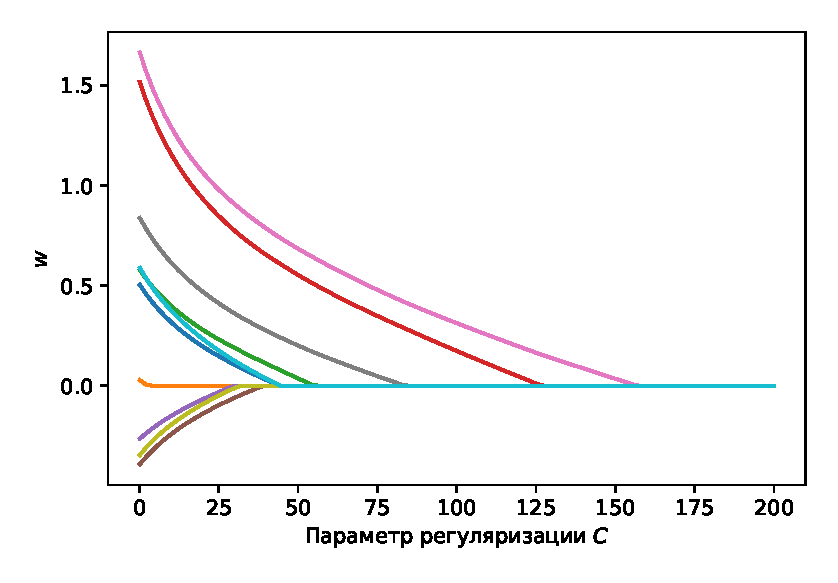
\includegraphics[width=0.5\textwidth]{../figures/log_reg_cs_exp.eps}
	\caption{Sample figure caption.}
	\label{fig:fig1}
\end{figure}

\subsection{Tables}
See awesome Table~\ref{tab:table}.

The documentation for \verb+booktabs+ (`Publication quality tables in LaTeX') is available from:
\begin{center}
	\url{https://www.ctan.org/pkg/booktabs}
\end{center}


\begin{table}
	\caption{Sample table title}
	\centering
	\begin{tabular}{lll}
		\toprule
		\multicolumn{2}{c}{Part}                   \\
		\cmidrule(r){1-2}
		Name     & Description     & Size ($\mu$m) \\
		\midrule
		Dendrite & Input terminal  & $\sim$100     \\
		Axon     & Output terminal & $\sim$10      \\
		Soma     & Cell body       & up to $10^6$  \\
		\bottomrule
	\end{tabular}
	\label{tab:table}
\end{table}

\subsection{Lists}
\begin{itemize}
	\item Lorem ipsum dolor sit amet
	\item consectetur adipiscing elit.
	\item Aliquam dignissim blandit est, in dictum tortor gravida eget. In ac rutrum magna.
\end{itemize}
\end{comment}

\bibliographystyle{unsrtnat}
\bibliography{references}

\end{document}
